\chapter{Searching for a good model}

\section{The Data}

The aim of this thesis is to use deep learning techniques to segment CT scans of the chest and identify the voxels that are in the part of the heart called the atrium. The atrium is composed of two chambers called the right and left atrium which are the two entry points of the blood into the heart, one returning to the heart to complete the circulating cycle through the body and the other coming back from the lungs after being oxygenated.\\

The data from which the training and testing datasets are generated comprise 27 chest computerised tomography (CT) scans. CT scans are 3 dimensional grey scale images generated via computers combining many X-ray images taken from different angles to produce cross-sectional images of specific body parts. They are stored as DICOM files, DICOM standing for Digital Imaging and Communications in Medicine and which is a standard for handling, storing, printing, and transmitting information in medical imaging. Each has been segmented by trained radiologists at St Thomas's hospital, the results of which are stored in Nearly Raw Raster Data (NRRD) files, a standard format for storing raster data. These are 3D arrays of the same dimension, each voxel taking either or two values which indicates whether the corresponding voxel in the CT scan is in the Atrium (1) or not (0). 

\section{Generating the datasets: The Tri-Planar Method}

Classifying the voxels require building an input set for each containing enough local and global information to allow the Neural Network to learn effectively. One way of providing 3 dimensional information is to use the so-called tri-planar method [reference the paper that started it on knee cartilage]. This consists in generating 3 perpendicular square patches of a given dimension in the transversal, saggital and coronal planes centred at the voxel of interest (see the figure). This standard technique has been found to give competitive results compared to using 3D patches while being much more computationally and memory efficient. In addition, we use a multiscale approach where we add 3 more input channels composed of compressed patches that are originally 5 times larger than the above set of patches resized to the same size to provide global information about the surroundings of concerned voxel.\\

Each patch is fed into a different input channel of the Convolutional Neural Network with one or more convolutional layers. The outputs of those channels are then feed as input to a number of connected layers before a classifying layer as output layer.

\begin{figure}
\centering
\begin{minipage}{0.45\textwidth}
\centering
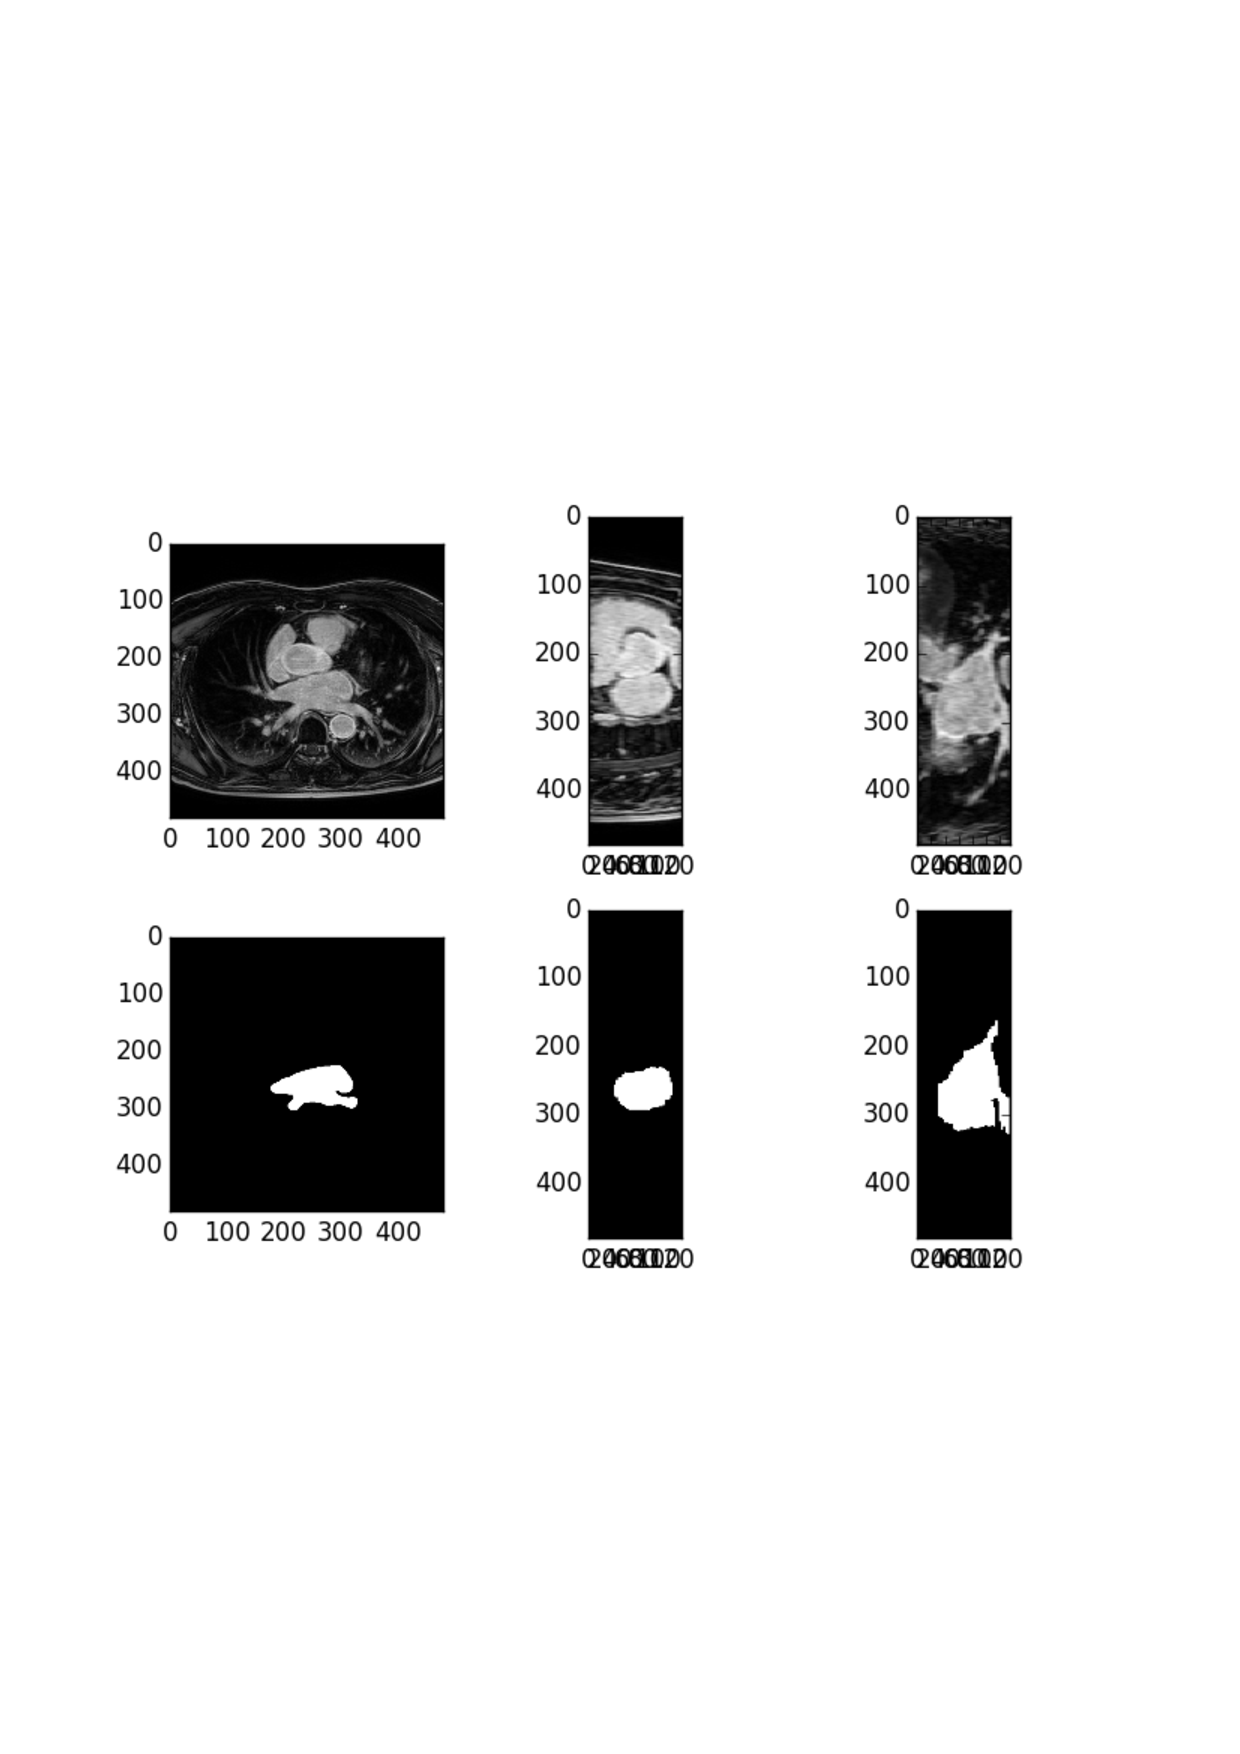
\includegraphics[trim=2cm 8cm 2cm 8cm, clip=true, height=60mm]{Chapter2/example_slice.pdf}
\end{minipage}\hfill
\begin{minipage}{0.45\textwidth}
\centering
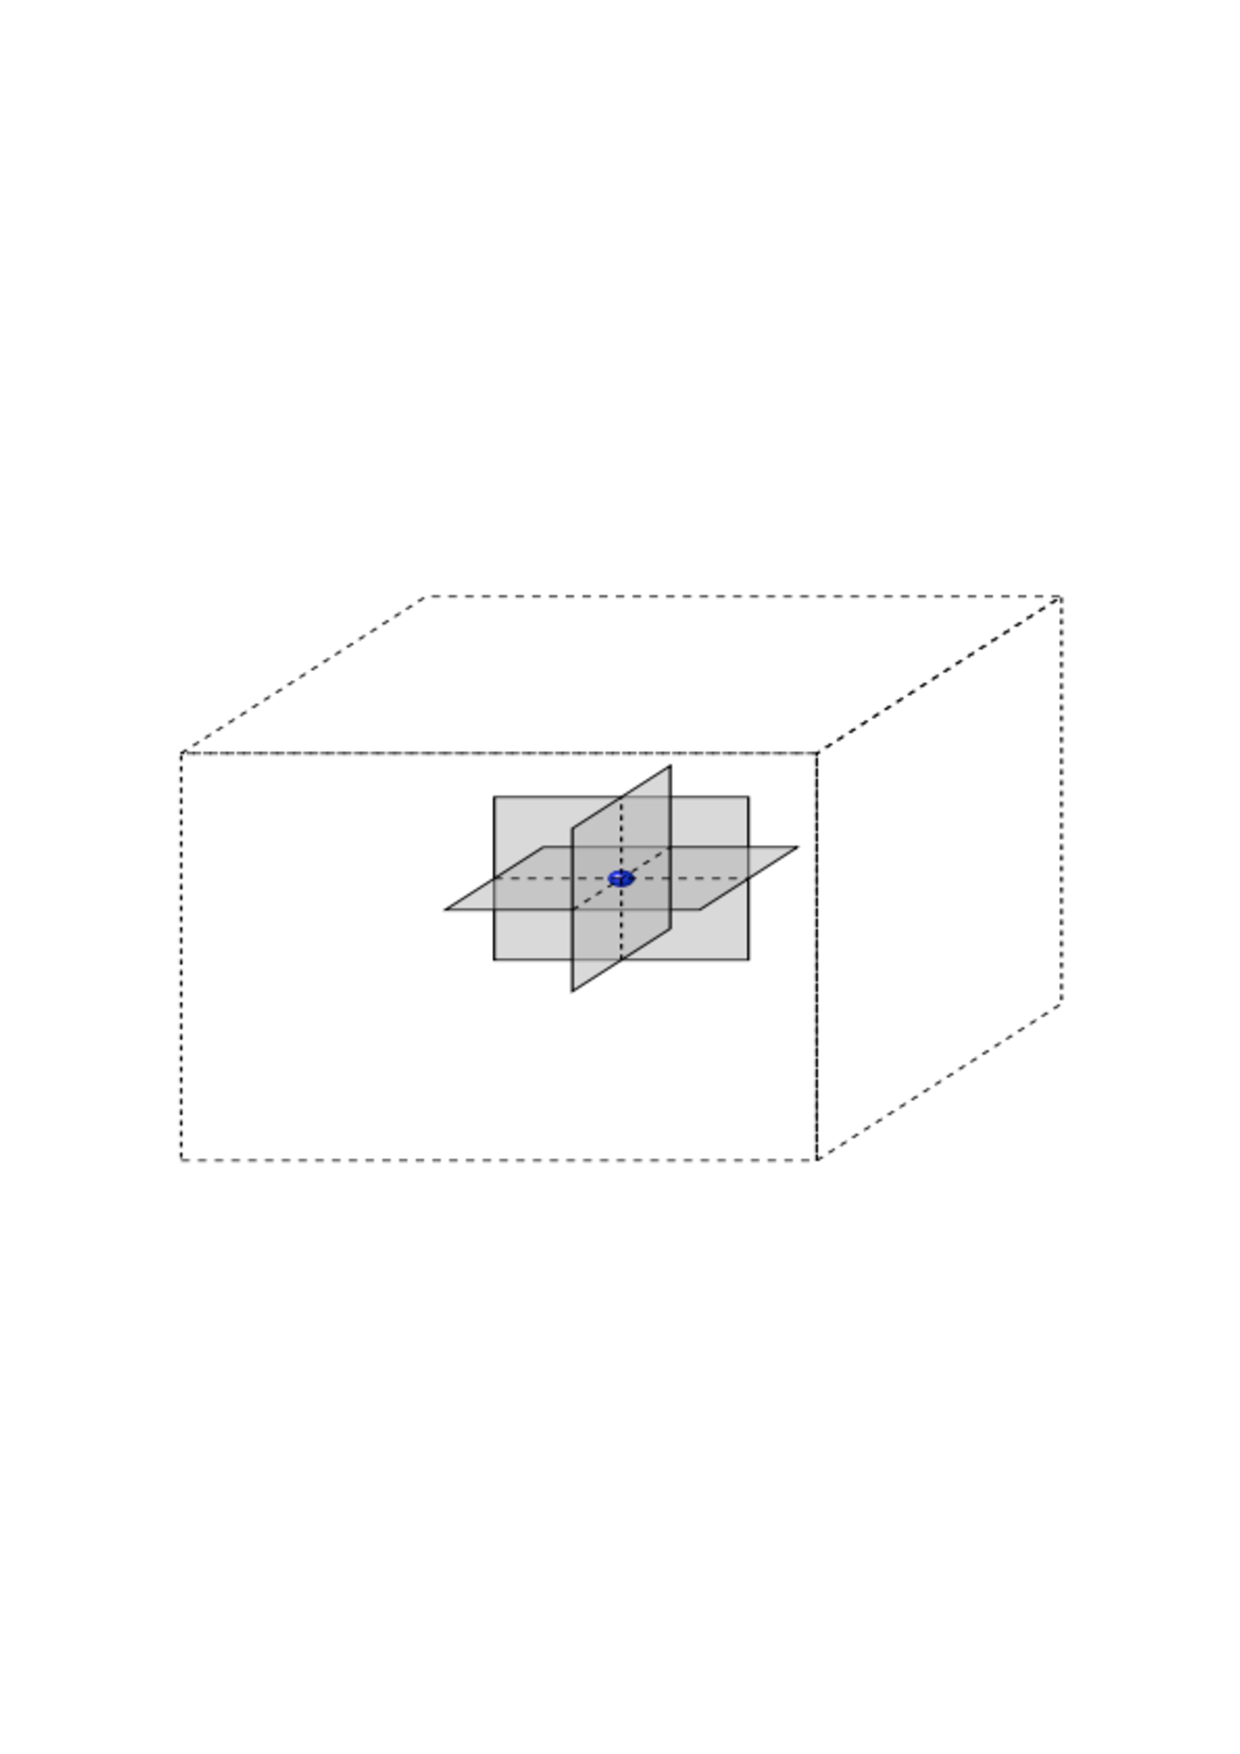
\includegraphics[trim=2cm 8cm 2cm 8cm, clip=true, height=60mm]{Chapter2/triplanar.pdf}
\end{minipage}
\caption{Left: grey scale slices from a CT scan taken in the transversal, saggital and coronal planes. Right: illustration of the triplanar}
\end{figure}

\section{Implementation Details}

\subsection{Libraries}

We use Torch, an open-source library maintained by Facebook in Lua aiming to provide a Matlab-like environment for scientific computing, along with a number of dependent libraries (cunn, cudnn, fbcunn) to train the convolutional networks on single and multi-GPUs. In addition, we use Python and a number of its libraries to handle all the logistics from generating the datasets to producing plots of segmentation results.

\subsection{Computer Power}

The training of the CNNs were conducted on 2 multi-GPU clusters, named montana-nvidia and montana-k80, kindly provided by Prof. Montana's laboratory. montana-nvidia consists 24 cores with 129 Gb of memory connected to two NVIDIA Tesla K40m and two Tesla K20Xm while montana-k80 on the other hand has 56 cores with 258 Gb of memory supported by 8 of NVIDIA's Testla K80. 

\section{Model Selection}

\subsection{General approach for model selection}

To look for a good model, we allocated 20 of the 27 CT scans to the training set, 7 to a testing set. We generated 400000 training examples equally divided among the training CT scans, half being in the atrium and the other half in the non-atrium part. The validation set is composed of 15000 testing examples from each testing CT scans to a total number of 105000 testing examples. The model selection is done by comparing the dice coefficient on the testing set calculated at the end of end epoch, which is just the classification accuracy in a 2-class problem, segmentation results from a few slices taken from the testing set and a final dice coefficient of the classification accuracy of the segmentation of the entire 7 testing CT scans preformed at the end of training.\\

We start off our model selection with a CNN composed of 2 convolutional layers with 32 and 64 feature maps respectively, 2 fully connected layers with 1000 and 500 hidden units each respectively, a logsoftmax output layer giving log probabilities. We will be varying in turn the following hyperparameters while keeping the rest constant.\\

\begin{itemize}
	\item varying the type of sampling method for the training set.
	\item varying the number of convolutional layers.
	\item varying the number of connected layers.
	\item varying the number of feature maps in the chosen number of convolutional layers.
	\item varying the number of hidden units in the chosen number of connected layers.
	\item varying the type of activation function (ReLU, Tanh or Sigmoid).
	\item varying the type of subsampling function (Maxpooling or average pooling).
	\item varying the learning rate.
	\item varying the momentum.
	\item varying the dataset size for the selected model.
\end{itemize}

\subsection{varying datasets type}

The first thing we investigate is the sampling method for obtaining the training set. In order to increase the number of non-atrium training examples lying near the boundaries where we expect most of the classification errors to lie, we construct a rectangular area which contains the atrium. The atrium box is constructed by going through all the coordinates of the voxels labeled as being in the atrium, picking the minimum and maximum values in each of the coordinate planes, and possibly adding some padding, this procedure gives us a box containing the atrium. \\

We train our base CNN on 3 sampling procedures with no atrium box, i.e. all the non-atrium training examples are sampled randomly uniformly, a small atrium box constructed by the procedure above with a padding of 5 pixels in the x and y coordinate directions and of 1 pixel in the z coordinate direction, and finally a large atrium box with a padding of 30 pixels in the x and y coordinates and of 5 pixels in the z coordinate.\\

The results of the three training runs are shown in Figure whatever. From the testing dice coefficient plot, we get a better classification rate with sampling using an atrium box than no atrium box and particularly with the smaller atrium box. In the segmentation mask, sampling with no atrium box clearly yields more errors in the proximity of the atrium but none away from it whereas there are some errors far away from the atrium from the models trained with the atrium box sampling procedure. This is a consequence of the sampling procedures in both cases. Sampling with an atrium box would naturally yield better segmentation results near the atrium as the proportion of training examples is much higher in those regions than without an atrium box around it.\\

\begin{figure}
\centering
\begin{minipage}{0.45\textwidth}
\centering
\fbox{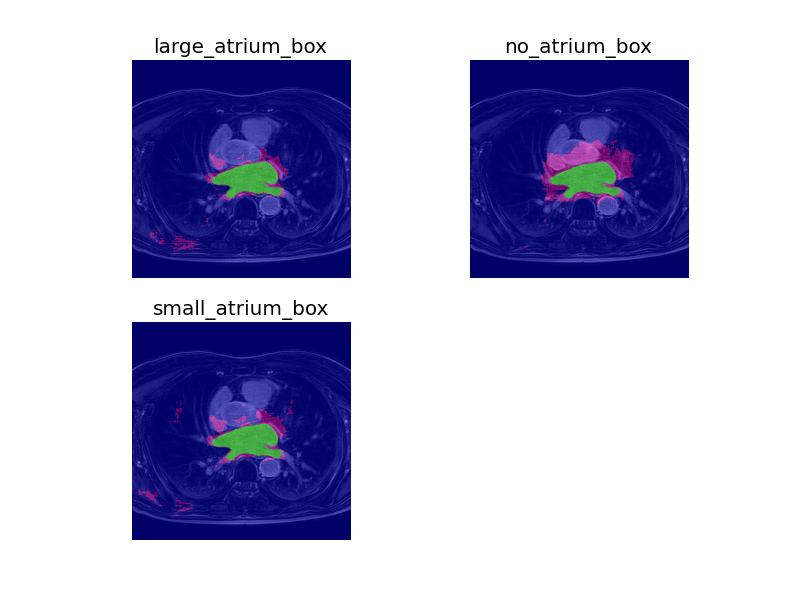
\includegraphics[trim=3cm 2cm 3cm 2cm, clip=true, height=60mm, width=70mm]{Chapter3/mask_results_varying_datasets.png}}
\end{minipage}\hfill
\hspace{-1cm}
\begin{minipage}{0.45\textwidth}
\centering
\fbox{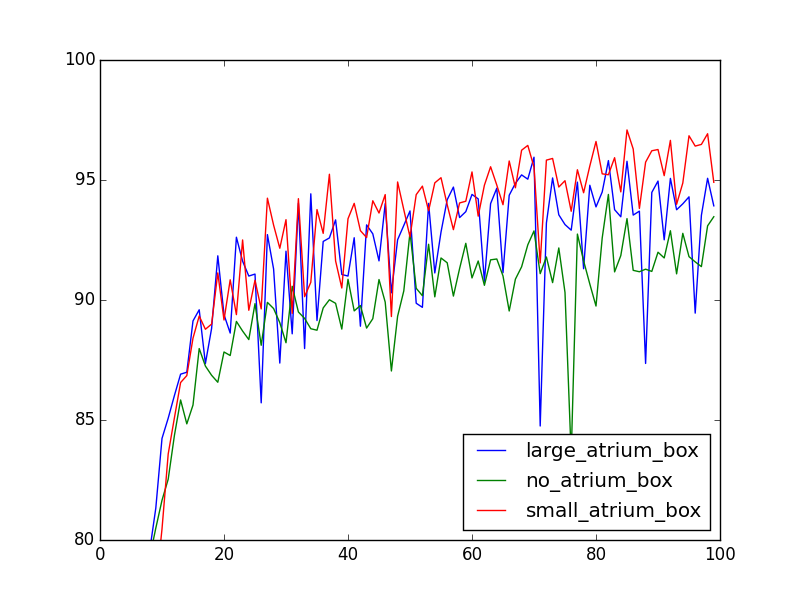
\includegraphics[trim=1cm 1cm 1cm 1cm, clip=true, height=60mm, width=70mm]{Chapter3/test_dice_coefficient_plots_varying_dataset.png}}
\end{minipage}
\caption{Right: test classification rate vs epoch number for the CNN trained with the 3 different sampling procedures. Left: segmentation result of a reference slice of one of the test CT scans for each of the models.}
\end{figure}

\subsection{varying number of convolutional layers}

Having established our sampling procedure, we now start the first step of our model selection: the number of convolutional layers. We train our CNN with the following 4 different architectures for the convolutional parts:

\begin{itemize}
	\item Input (6*32*32) => Conv layer (32*28*28) => 2*2 MaxPooling filter (32*14*14) 
	\item Input (6*32*32) => Conv layer (32*28*28) => 2*2 MaxPooling filter (32*14*14) => Conv layer (64*10*10) => 2*2 MaxPooling filter (64*5*5)
	\item Input (6*32*32) => Conv layer (32*28*28) => Conv layer (32*24*24) => 2*2 MaxPooling filter (32*12*12) => Conv layer (64*8*8) => 2*2 MaxPooling filter (64*4*4)
	\item Input (6*32*32) => Conv layer (32*28*28) => Conv layer (32*24*24) => 2*2 MaxPooling filter (32*12*12) => Conv layer (64*8*8) => Conv layer (64*4*4) => 2*2 MaxPooling filter (64*2*2)
\end{itemize}

Each of those architectures is then followed by the same fully connected layers as used for selecting the sampling procedure. We find that having more than 1 doesn't improve the results much. 

\begin{figure}
\centering
\begin{minipage}{0.45\textwidth}
\centering
\fbox{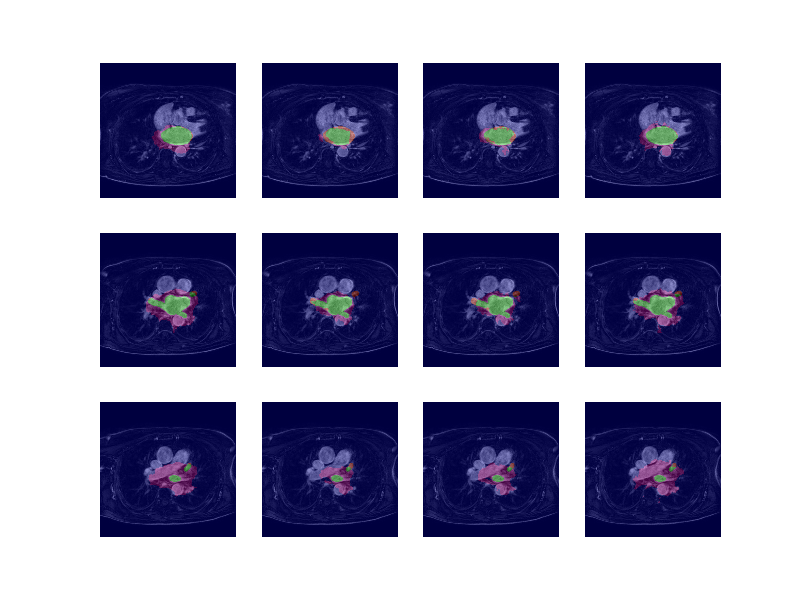
\includegraphics[trim=3cm 2cm 3cm 2cm, clip=true, height=60mm, width=70mm]{Chapter3/mask_results_varying_number_of_convolutional_layers.png}}
\end{minipage}\hfill
\hspace{-1cm}
\begin{minipage}{0.45\textwidth}
\centering
\fbox{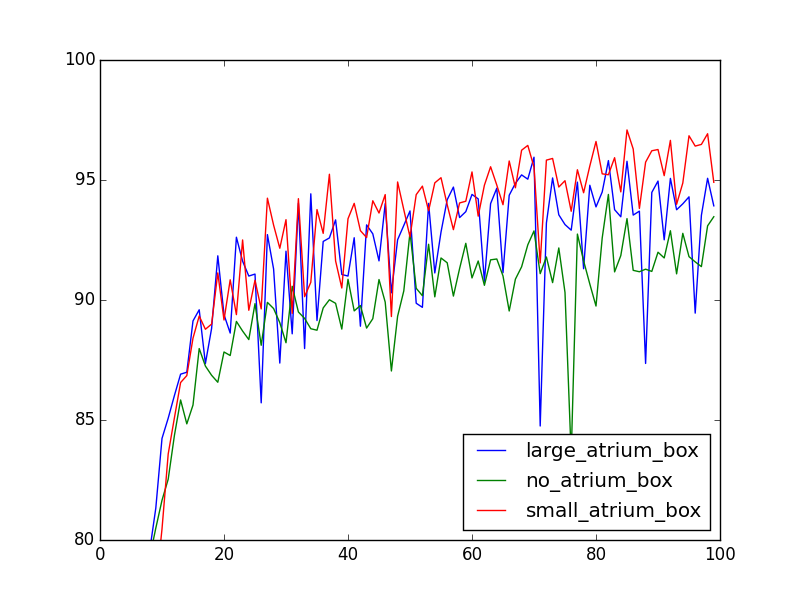
\includegraphics[height=60mm, width=70mm]{Chapter3/test_dice_coefficient_plots_varying_dataset.png}}
\end{minipage}
\caption{Left: grey scale slices from a CT scan taken in the transversal, saggital and coronal planes. Right: illustration of the triplanar}
\end{figure}

\subsection{varying number of connected layers}

Having settled on an architecture with 1 convolutional layer, we trained 3 CNNs with 1, 2, and 3 connected layers each having 1000 hidden units. Having more than 1 connected layer doesn't make a difference.

\begin{figure}
\centering
\begin{minipage}{0.45\textwidth}
\centering
\fbox{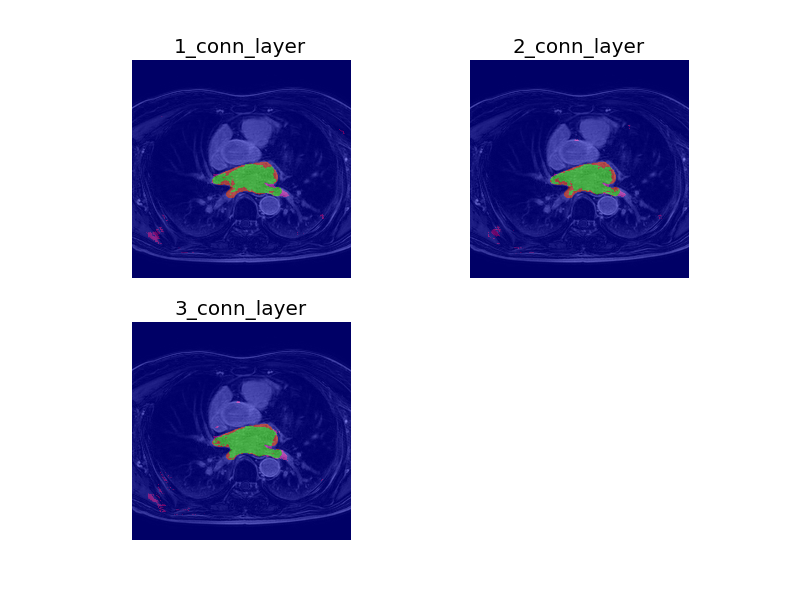
\includegraphics[trim=3cm 2cm 3cm 2cm, clip=true, height=60mm, width=70mm]{Chapter3/mask_results_varying_number_of_connected_layers.png}}
\end{minipage}\hfill
\hspace{-1cm}
\begin{minipage}{0.45\textwidth}
\centering
\fbox{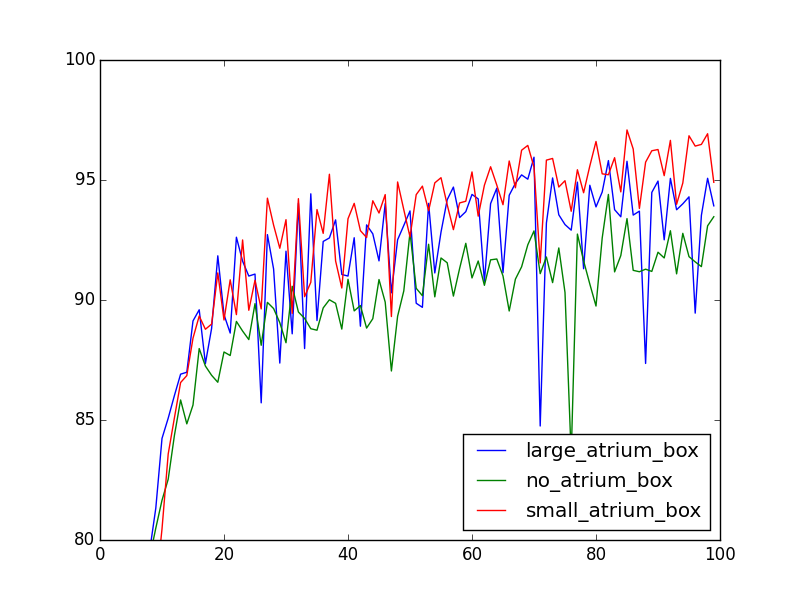
\includegraphics[height=60mm, width=70mm]{Chapter3/test_dice_coefficient_plots_varying_dataset.png}}
\end{minipage}
\caption{Left: grey scale slices from a CT scan taken in the transversal, saggital and coronal planes. Right: illustration of the triplanar}
\end{figure}

\subsection{varying number of feature maps}

So now the focus is on finding the right number of feature maps for the convolutional layer. We tried 16/32/64/128 and it seems having 64 feature maps gives the best bang for the buck.

\begin{figure}
\centering
\begin{minipage}{0.45\textwidth}
\centering
\fbox{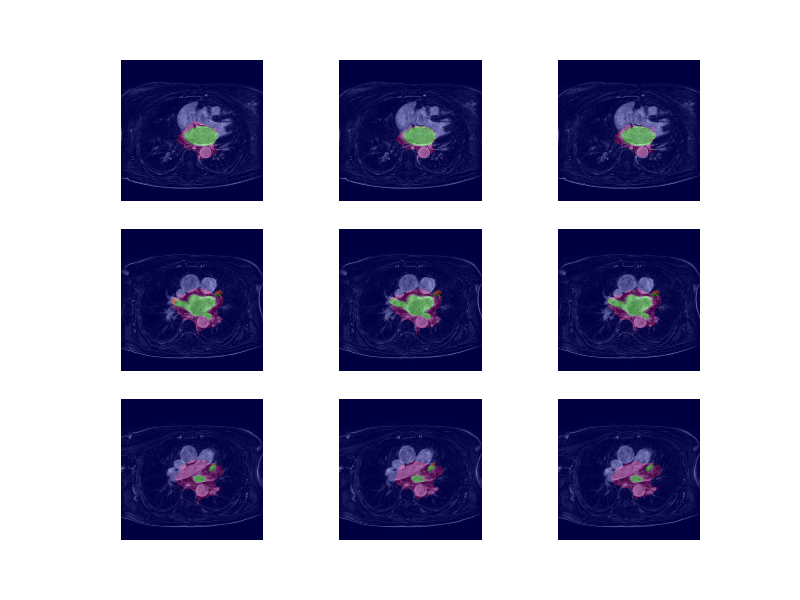
\includegraphics[trim=3cm 2cm 3cm 2cm, clip=true, height=60mm, width=70mm]{Chapter3/mask_results_varying_number_of_feature_maps.png}}
\end{minipage}\hfill
\hspace{-1cm}
\begin{minipage}{0.45\textwidth}
\centering
\fbox{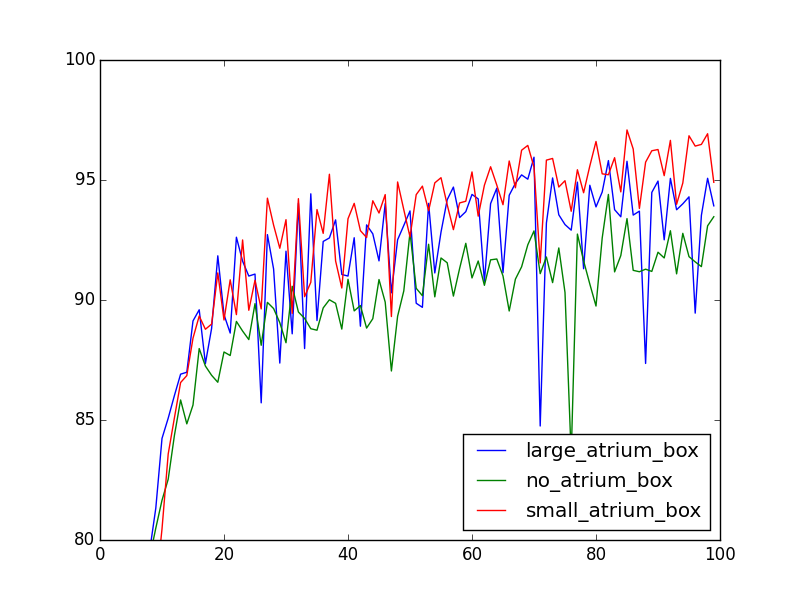
\includegraphics[height=60mm, width=70mm]{Chapter3/test_dice_coefficient_plots_varying_dataset.png}}
\end{minipage}
\caption{Left: grey scale slices from a CT scan taken in the transversal, saggital and coronal planes. Right: illustration of the triplanar}
\end{figure}

\subsection{varying the number of hidden units}

We now vary the number of hidden units in the connected layer, trying 100, 200, 500, 1000 and 1500. 200 is best...

\begin{figure}
\centering
\begin{minipage}{0.45\textwidth}
\centering
\fbox{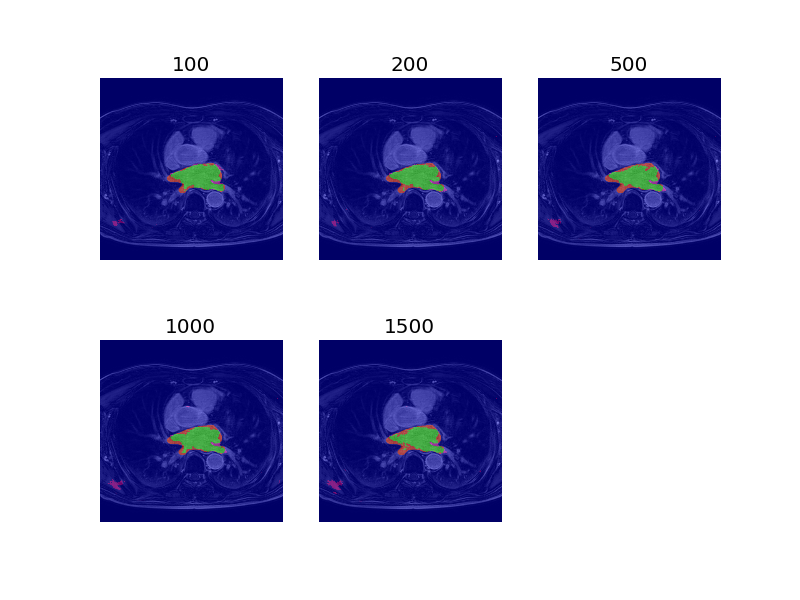
\includegraphics[trim=3cm 2cm 3cm 2cm, clip=true, height=60mm, width=70mm]{Chapter3/mask_results_varying_number_of_connected_hidden_units.png}}
\end{minipage}\hfill
\hspace{-1cm}
\begin{minipage}{0.45\textwidth}
\centering
\fbox{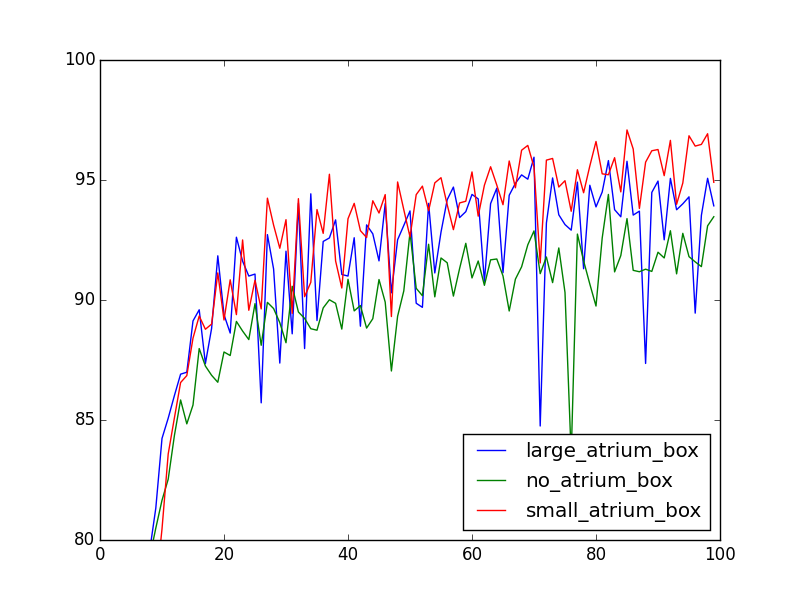
\includegraphics[height=60mm, width=70mm]{Chapter3/test_dice_coefficient_plots_varying_dataset.png}}
\end{minipage}
\caption{Left: grey scale slices from a CT scan taken in the transversal, saggital and coronal planes. Right: illustration of the triplanar}
\end{figure}

\subsection{varying the activation function}

We experimented with different types of activation function: ReLU, Tanh, Sigmoid. Doing it with ReLU is better...

\begin{figure}
\centering
\begin{minipage}{0.45\textwidth}
\centering
\fbox{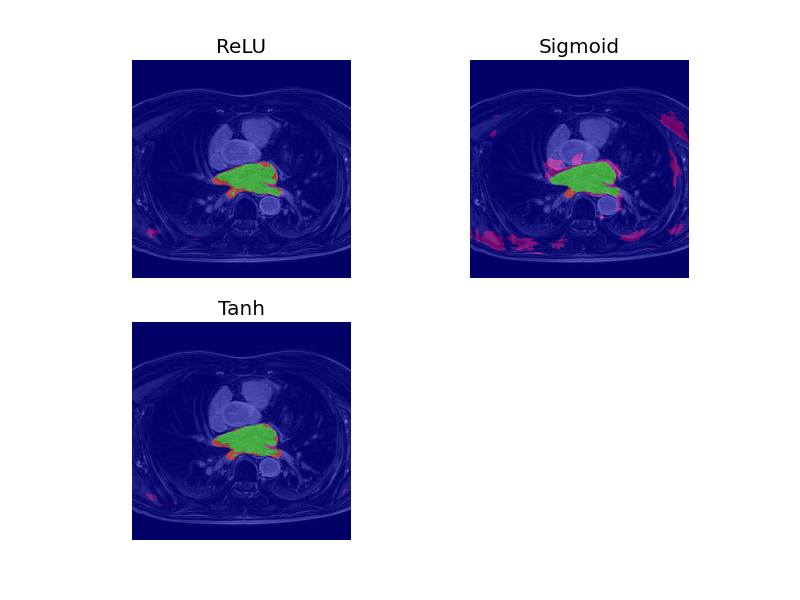
\includegraphics[trim=3cm 2cm 3cm 2cm, clip=true, height=60mm, width=70mm]{Chapter3/mask_results_varying_activation_functions.png}}
\end{minipage}\hfill
\hspace{-1cm}
\begin{minipage}{0.45\textwidth}
\centering
\fbox{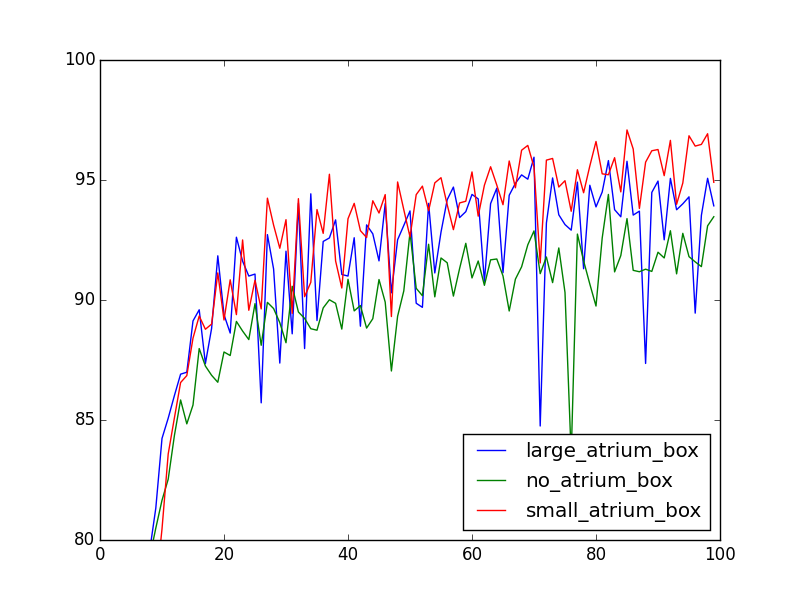
\includegraphics[height=60mm, width=70mm]{Chapter3/test_dice_coefficient_plots_varying_dataset.png}}
\end{minipage}
\caption{Left: grey scale slices from a CT scan taken in the transversal, saggital and coronal planes. Right: illustration of the triplanar}
\end{figure}


\subsection{varying the type of pooling}

We also tried different types of pooling: Max pooling and average pooling. No difference, so we stuck with Max pooling

\begin{figure}
\centering
\begin{minipage}{0.45\textwidth}
\centering
\fbox{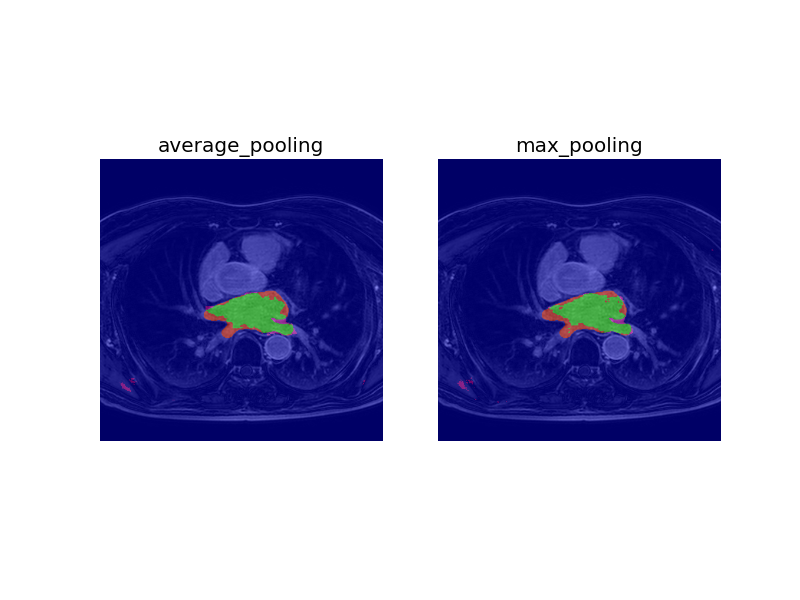
\includegraphics[trim=3cm 2cm 3cm 2cm, clip=true, height=60mm, width=70mm]{Chapter3/mask_results_varying_pooling_functions.png}}
\end{minipage}\hfill
\hspace{-1cm}
\begin{minipage}{0.45\textwidth}
\centering
\fbox{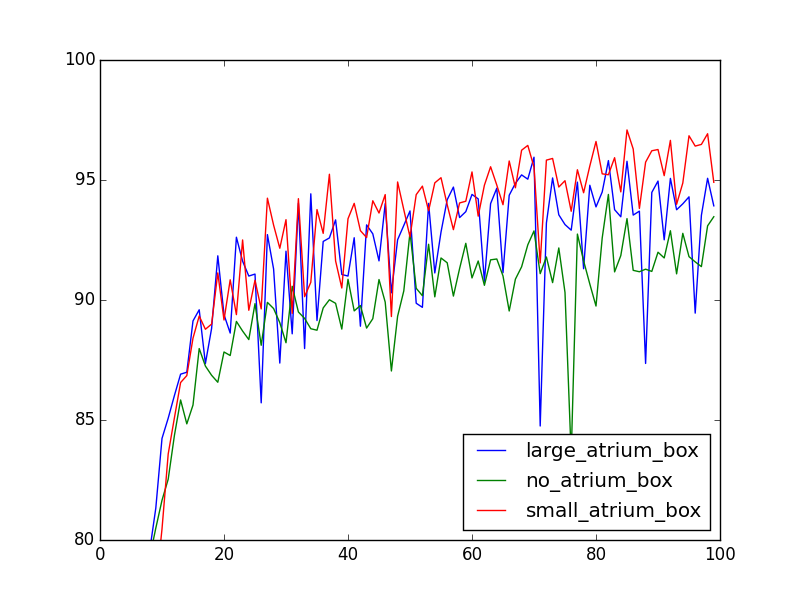
\includegraphics[height=60mm, width=70mm]{Chapter3/test_dice_coefficient_plots_varying_dataset.png}}
\end{minipage}
\caption{Left: grey scale slices from a CT scan taken in the transversal, saggital and coronal planes. Right: illustration of the triplanar}
\end{figure}


\subsection{varying the learning rate}

Tried different learning rates: 0.01, 0.05, 0.1, 0.5, 1. It seems that 0.1 is best. Having a learning rate of 1 doesn't train the network.  We omitted the results.

\begin{figure}
\centering
\begin{minipage}{0.45\textwidth}
\centering
\fbox{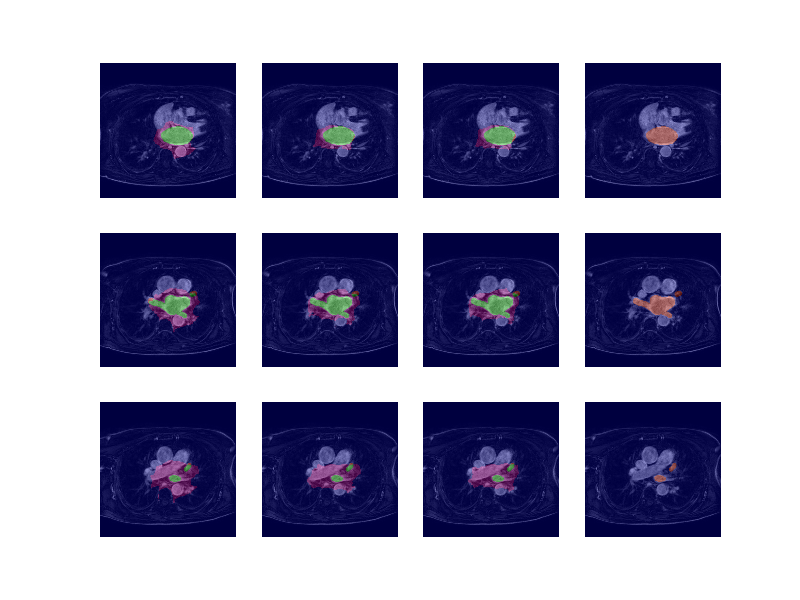
\includegraphics[trim=3cm 2cm 3cm 2cm, clip=true, height=60mm, width=70mm]{Chapter3/mask_results_varying_learning_rate.png}}
\end{minipage}\hfill
\hspace{-1cm}
\begin{minipage}{0.45\textwidth}
\centering
\fbox{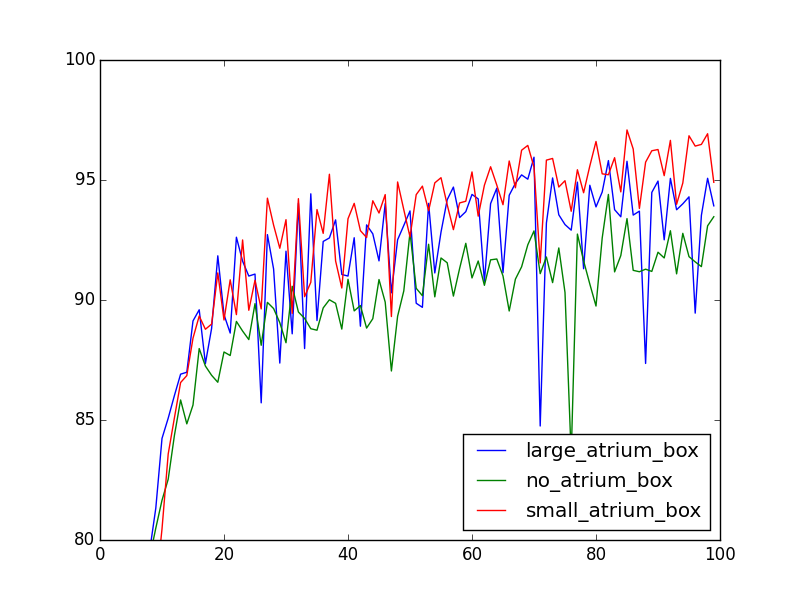
\includegraphics[height=60mm, width=70mm]{Chapter3/test_dice_coefficient_plots_varying_dataset.png}}
\end{minipage}
\caption{Left: grey scale slices from a CT scan taken in the transversal, saggital and coronal planes. Right: illustration of the triplanar}
\end{figure}

\subsection{varying the momentum}

Tried different momentums: 0, 0.01, 0.05, 0.1. Having momentum actually slightly improves the test results!

\begin{figure}
\centering
\begin{minipage}{0.45\textwidth}
\centering
\fbox{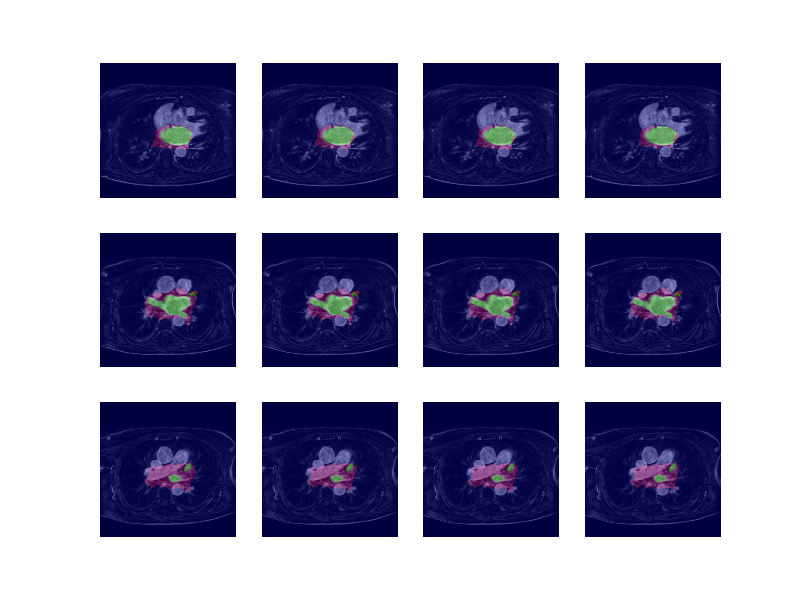
\includegraphics[trim=3cm 2cm 3cm 2cm, clip=true, height=60mm, width=70mm]{Chapter3/mask_results_varying_momentum.png}}
\end{minipage}\hfill
\hspace{-1cm}
\begin{minipage}{0.45\textwidth}
\centering
\fbox{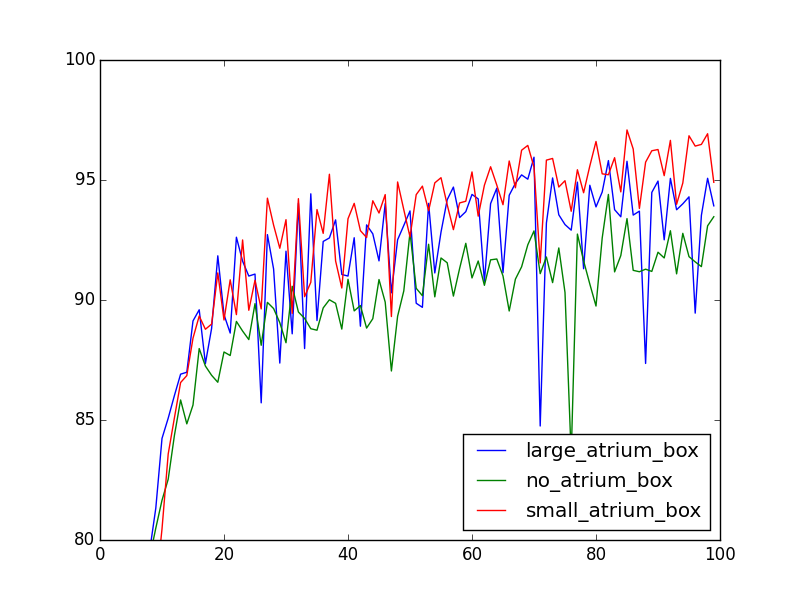
\includegraphics[height=60mm, width=70mm]{Chapter3/test_dice_coefficient_plots_varying_dataset.png}}
\end{minipage}
\caption{Left: grey scale slices from a CT scan taken in the transversal, saggital and coronal planes. Right: illustration of the triplanar}
\end{figure}

\subsection{varying the data size}

Tried a number of dataset sizes: 400000, 1000000, 3000000: No improved result from the increased data size.


